% !TXS template
\documentclass[titlepage]{article}
\usepackage[utf8]{inputenc}
\usepackage{color}   %May be necessary if you want to color links
\usepackage{hyperref}
\usepackage[french]{babel}
\usepackage{cite}
\usepackage{graphicx}

\hypersetup{
	colorlinks=true, %set true if you want colored links
	linktoc=all,     %set to all if you want both subsections and subsubsections linked
	linkcolor=blue,  %choose some color if you want links to stand out
}
\title{Arbre comportementaux pour le contr\^ole de mission}
\author{
	Derrien Martial \\
	\and
	Madec Antoine \\
	\and
	Lucas Florian
}
\date{Juin 2019}
\renewcommand{\contentsname}{Sommaire} 
\begin{document}
	\maketitle
	\tableofcontents
	\hypersetup{linktocpage}
	
	\clearpage
	\section{Introduction}
	Un arbre comportemental (Behavior Tree, BT en anglais) est une
	technique permettant de structurer le passage d'une tâche à une autre dans 
	le cadre de l'automatisation de ce comportement.
	\\
	Cette technique, d'abord utilisé pour programmer le comportement de personnages non joueurs (NPC) dans les jeux vidéos \cite{wikipedia_BT}, est maintenant l'une des techniques les plus en vogue pour la programmation de robot autonome ou semi-autonome\cite{ros.org}.
	\\
	\begin{figure}[h!]
		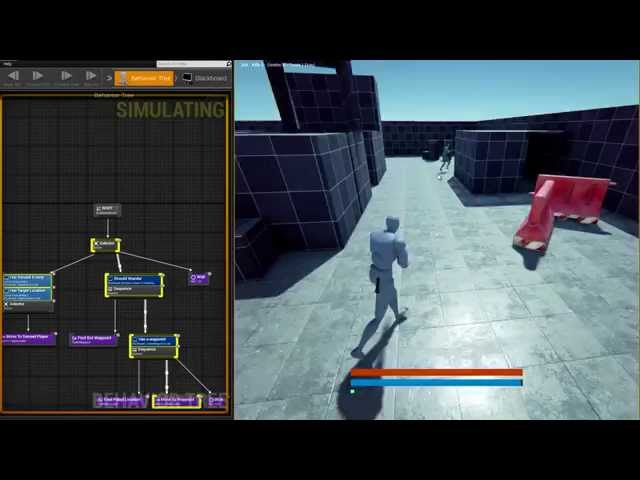
\includegraphics[width=\linewidth]{img/videogame_tree.jpg}
		\caption{Conception d'un jeu vidéo utilisant les BT}
		\label{fig:BT2}
	\end{figure}
	\\
	L'objectif de ce rapport est de faire une synthèse de l'utilisation émergente des BT en robotique, et ce dans de multiples domaines.
	\\
	Tout d'abord, nous allons définir ce qu'est un BT et quelles sont ses utilisations historiques. Ensuite, nous verrons qu'elles sont les nouvelles applications de cette technique dans les domaines variés de la robotique. Enfin, nous décrirons une implémentation simple d'un BT dans un projet de robotique théorique.
	\clearpage
	\section{Qu'est-ce-qu'un behavior tree ?}
		\subsection{Définition}
		Un arbre de comportement est un modèle mathématique d'exécution de plans utilisé en informatique, en robotique, en systèmes de contrôle et dans les jeux vidéo. Ils décrivent les basculements entre un ensemble fini de tâches de manière modulaire. Leur force provient de leur capacité à créer des tâches très complexes composées de tâches simples, sans se soucier de la façon dont les tâches simples sont mises en œuvre. \cite{wikipedia_BT}
		\subsection{fonctionnement}
		
		D'un point de vue conceptuel, un BT est basé sur deux objets clés : le nœud et l'arborescence.
		
		\begin{figure}[h!]
			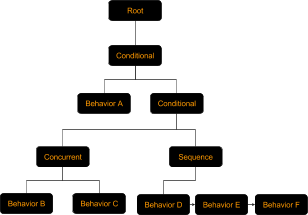
\includegraphics[width=\linewidth]{img/behavior_trees_example.png}
			\caption{exemple de BT \cite{rasmussen}}
			\label{fig:BT1}
		\end{figure}
		
		\paragraph{Nœud}
		Le nœud est le concept le plus fondamental ici. il s'agit d'un bloc de construction qui peut être associé à d'autres pour construire des comportements. Un nœud se compose d'un bloc de code qui représente une tâche simple. Tous les nœuds ont la même interface : lors de leur traitement, ils effectuent une tâche et peuvent réussir ou échouer.
		
		Les nœuds peuvent être autonomes ou avoir des nœuds enfants, lesquels sont traités dans le cadre du traitement du nœud parent. Lors du traitement, la réussite d'un nœud parent dépend souvent (mais pas toujours) de la réussite de chaque nœud enfant.
		
		Les nœuds suivent plusieurs modèles courants, tels que les nœuds d'action, composites et décorateurs. \cite{documentation_aws}
		
		\paragraph{Arborescence}
		Les comportements sont élaborés en construisant des arborescences de nœuds, collections de tâches individuelles qui, lorsqu'elles sont positionnées comme une racine avec des branches qui se terminent par des feuilles, définissent la façon dont un agent intelligent se comportera en réponse à une entrée. \cite{documentation_aws}	
		\subsection{historique}
			D'un point de vue théorique, chaque exécution décrite par un BT peut être décrite par un FSM et inversement [34, 46]. Toutefois, en raison du nombre de transitions, l'utilisation d'un FSM en tant qu'AC n'est pas pratique pour certaines applications robotiques. De plus, un FSM suppose que les propositions qui déclenchent les transitions sortantes à partir du même état s’excluent mutuellement. Une fois mises en œuvre, les propositions sont vérifiées régulièrement en un temps discret. Il existe donc une probabilité non nulle que deux propositions ou plus se tiennent simultanément après un cycle. Pour résoudre ce problème, nous devons redéfinir la signification de certaines transitions, comme indiqué dans l’FSM de la Figure 1.3, rendant les propositions des transitions sortantes mutuellement exclusives. Un FSM de ce format est peu pratique à concevoir pour les humains et les ordinateurs. Ajouter et supprimer des comportements humains est sujet à des erreurs. Après avoir ajouté un nouvel état, chaque transition existante doit être réévaluée (éventuellement supprimée ou remplacée) et les nouvelles transitions depuis / vers le nouvel état doivent également être évaluées. Un grand nombre de transitions rend tout processus automatisé d'analyse ou de synthèse coûteux en FSM.
			Les HFSM sont les autorités de certification les plus similaires aux BT en termes d'objectif et d'expressivité. Pour comparer les BT aux HFSM, veuillez vous référer à \cite{colledanchise_2017}. Une différence importante est que, dans les HFSM, chaque couche de la hiérarchie doit être ajoutée explicitement, alors que dans les BT, chaque sous-arbre peut être vu comme un module à part entière, avec la même interface qu'une action atomique.
			Dans le HFSM illustré à la figure 3.8, une proposition doit être fournie pour chaque transition. Pour améliorer la lisibilité, nous avons numéroté ces propositions de C1 à C10. La couche supérieure du HFSM contient les sous-HFSM de l'autoprotection et des activités performantes. À l'intérieur de ce dernier, nous avons deux sous-HFSM parallèles. L’une traite l’interaction de l’utilisateur, tandis que la plus grande contient un graphe orienté complet gérant la commutation entre les différentes activités. Enfin, Play Ball Game est un autre sous-HFSM avec le suivi de la balle exécuté en parallèle avec un autre graphe dirigé complet, gérant le basculement réactif entre la balle d’approche, la balle à saisir et la balle au lancer.
			Les deux figures montrent clairement comment la modularité est gérée par le HFSM. Le sous-HFSM explicitement défini encapsule l'autoprotection, l'exécution d'activités et le jeu de balle. Cependant, à l'intérieur de ces sous-HFSM, la structure de transition est un graphe dirigé complet, avec n (n != 1) transitions à conserver (n étant le nombre de nœuds).
			En examinant les logiciels disponibles pour la conception et l'exécution de FSM et de BT, nous constatons que les outils du côté FSM, tels que IBM Rhapsody 2 et Stateflow 3, sont beaucoup plus avancés. Néanmoins, de nombreuses plates-formes de développement de jeux informatiques, telles que Unity3d 4 et Unreal Engine 5, disposent désormais d'outils permettant de travailler avec des BT. Pour ceux qui souhaitent mettre en œuvre leur propre cadre, nous notons que la mise en œuvre standard des FSM est assez simple, alors que les HFSM et les BT nécessitent davantage de considération. Cependant, les implémentations open source sont disponibles pour les deux. 6,7 Enfin, dans [A], nous comparons les BT avec les DT; l'architecture de subsomption; et la composition séquentielle. Dans [B], nous comparons les BT avec les arbres AND-OR et les programmes TR.
	\begin{figure}[h!]
		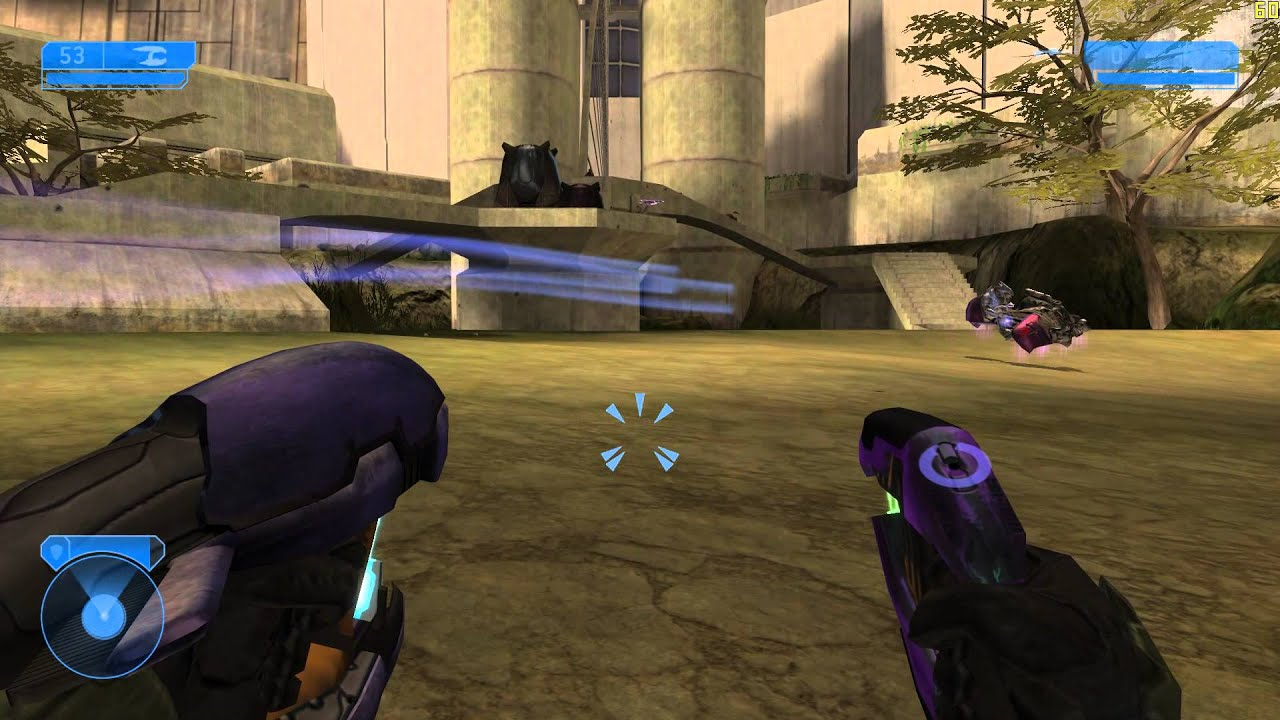
\includegraphics[width=\linewidth]{img/halo2.jpg}
		\caption{Le jeu vidéo Halo2, un précurseur en matière d'intelligence artificielle dans le jeu vidéo grâce à son utilisation des BT \cite{wikipedia_halo}}
		\label{fig:BT1}
	\end{figure}
	
	\clearpage
	\section{Les behavior tree en robotique}
		\subsection{civil}
	
		\subsection{industrie}
	
		\subsection{santé}
	prédire comportement
	
		\subsection{militaire}
	prédire comptmt
	
	\clearpage
	\section{Les outils implémentant les behavior trees}
		\subsection{outils utilisés}
		\subsection{outils incomplet}
		\subsection{machine learning}
		Dans la définition originale de l’arbre de comportement, les sélecteurs choisiront l’un de leurs nœuds-enfants à valider. L’algorithme parcourant l'arbre de gauche à droite pour trouver le premier des noeuds pouvant être activé donne aux noeuds de gauche les poids les plus élevés. \cite{Fu2016/08}
		\\
		Cependant, une considération plus naturelle consiste à attacher le poids aux nœuds enfants. Les sélecteurs cochent leurs nœuds enfants conformément aux poids de haut en bas. Cependant, cela implique d'ajuster manuellement les valeurs de pondération pour le système. Ce qui implique beaucoup de main-d'œuvre et de ressources : c'est une tâche très compliquée et très lourde, pas vraiment immaginable sur un très gros projet. \cite{Fu2016/08}
		\\
		Une solution serait donc d'utiliser l'apprentissage machine (machine learning) afin de faire ajuster ces valeurs automatiquement.
	
	\clearpage
	\section{Exemple d'implémentation}
	
	\clearpage
	\section{bibliographie}
	\bibliographystyle{plain}
	\bibliography{sources.bib}
	
\end{document}
